\documentclass[12pt, twoside]{article}
\documentclass[12pt, twoside]{article}
\usepackage[letterpaper, margin=1in, headsep=0.2in]{geometry}
\setlength{\headheight}{0.6in}
%\usepackage[english]{babel}
\usepackage[utf8]{inputenc}
\usepackage{microtype}
\usepackage{amsmath}
\usepackage{amssymb}
%\usepackage{amsfonts}
\usepackage{siunitx} %units in math. eg 20\milli\meter
\usepackage{yhmath} % for arcs, overparenth command
\usepackage{tikz} %graphics
\usetikzlibrary{quotes, angles}
\usepackage{graphicx} %consider setting \graphicspath{{images/}}
\usepackage{parskip} %no paragraph indent
\usepackage{enumitem}
\usepackage{multicol}
\usepackage{venndiagram}

\usepackage{fancyhdr}
\pagestyle{fancy}
\fancyhf{}
\renewcommand{\headrulewidth}{0pt} % disable the underline of the header
\raggedbottom
\hfuzz=2mm %suppresses overfull box warnings

\usepackage{hyperref}
\usepackage{float}

\fancyhead[LE]{\thepage}
\fancyhead[RO]{\thepage \\ First and last name: \hspace{2.5cm} \,\\ Section: \hspace{2.5cm} \,}
\fancyhead[LO]{BECA / Dr. Huson / Regents Prep: Graphs\\* 30 October 2024}

\begin{document}

\subsubsection*{1.8 Do Now: Graphing lines and finding intersections}
\begin{enumerate}
  \item Graph and label the two equations. Mark their intersection as an ordered pair.

  \begin{multicols}{2}
    $y = \frac{1}{2}x-3$ \\[0.25cm]
    Write down the slope and $y$-intercept\\ of the first equation.
    \begin{enumerate}
      \item $m=$ \bigskip
      \item $b=$
    \end{enumerate}
    \columnbreak
    $2x+y = 7$ \\[0.5cm]
        Write as slope-intercept form, $y=mx+b$.
    \end{multicols}

  \begin{center} %4 quadrant regents grid w T-Chart
  \begin{tikzpicture}[scale=.635]
    \draw [help lines] (-10,-10) grid (10,10);
    \draw [thick, ->] (-10.2,0) -- (10.4,0) node [below right] {$x$};
    \draw [thick, ->] (0,-10.2)--(0,10.4) node [left] {$y$};
  \end{tikzpicture}
  \end{center}

\item Graph on the number line the inequality $x \geq -2$. \vspace{0.5cm}
  \begin{center}
    \begin{tikzpicture}
      \draw [thick, <->] (-5.4,0) -- (6.4,0) node [below right] {$x$};
      \foreach \x in {-5,-4,...,6}
        \draw[shift={(\x,0)}, thick] (0pt,3pt) -- (0pt,-3pt) node[below] {\x};
      %\draw[thick] (3,0) -- (-6,0);
    \end{tikzpicture}
    \end{center}

\newpage
\item Each quadratic equation has been factored as the first step to solve $x$. Complete each solution.
\begin{multicols}{2}
  \begin{enumerate}[itemsep=5cm]
    \item $x^2 + 5x - 6 = 0$ \\[0.5cm]
      Solution (first step): \\
      $(x + 6)(x - 1) = 0$
    \item $x^2 - 12x + 11 = 0$ \\[0.5cm]
      Solution (first step): \\
      $(x - 1)(x - 11) = 0$
    \end{enumerate}
    \end{multicols} \vspace{2cm}

\item Factor each equation and solve for the values of $x$.
  \begin{multicols}{2}
    \begin{enumerate}[itemsep=5cm]
    \item $x^2-5x+4=0$
    \item $x^2+7x+10=0$
  \end{enumerate}
  \end{multicols} \vspace{5cm}

Quadratic formula: For $ax^2+bx+c=0$, $\displaystyle x=\frac{-b \pm \sqrt{b^2-4ac}}{2a}$
\item Solve using the quadratic formula. (example given)
\begin{multicols}{2}
  \begin{enumerate}[itemsep=5cm]
    \item $2x^2 + 3x + 1 = 0$ \\[0.5cm]
    Solution:
      \begin{align*}
        x &= \frac{-3 \pm \sqrt{9 - 8}}{4} \\
        x &= \frac{-3 \pm \sqrt{1}}{4} \\
        x &= \frac{-3 \pm 1}{4} \\
        x &= \frac{-2}{4} \quad \text{or} \quad x = \frac{-4}{4} \\
        x &= -\frac{1}{2} \quad \text{or} \quad x = -1
      \end{align*}
      \item $3x^2 + 2x - 1 = 0$
  \end{enumerate}
  \end{multicols} \vspace{4cm}


\end{enumerate}
\end{document}